%%%%%%%%%%%%%%%%%%%%%%%%%%%%%%%%%%%%%%%%%
% Programming/Coding Assignment
% LaTeX Template
%
% This template has been downloaded from:
% http://www.latextemplates.com
%
% Original author:
% Ted Pavlic (http://www.tedpavlic.com)
%
% Note:
% The \lipsum[#] commands throughout this template generate dummy text
% to fill the template out. These commands should all be removed when 
% writing assignment content.
%
% This template uses a Perl script as an example snippet of code, most other
% languages are also usable. Configure them in the "CODE INCLUSION 
% CONFIGURATION" section.
%
%%%%%%%%%%%%%%%%%%%%%%%%%%%%%%%%%%%%%%%%%

%----------------------------------------------------------------------------------------
%	PACKAGES AND OTHER DOCUMENT CONFIGURATIONS
%----------------------------------------------------------------------------------------

\documentclass{article}

\usepackage{fancyhdr} % Required for custom headers
\usepackage{lastpage} % Required to determine the last page for the footer
\usepackage{extramarks} % Required for headers and footers
\usepackage[usenames,dvipsnames]{color} % Required for custom colors
\usepackage{graphicx} % Required to insert images
\usepackage{listings} % Required for insertion of code
\usepackage{courier} % Required for the courier font
\usepackage{lipsum} % Used for inserting dummy 'Lorem ipsum' text into the template
\usepackage{hyperref}
% Margins
\topmargin=-0.45in
\evensidemargin=0in
\oddsidemargin=0in
\textwidth=6.5in
\textheight=9.0in
\headsep=0.25in

\linespread{1.1} % Line spacing

% Set up the header and footer
\pagestyle{fancy}
\lhead{\hmwkAuthorName} % Top left header
\chead{\hmwkClass\ (\hmwkClassInstructor\ \hmwkClassTime): \hmwkTitle} % Top center head
\rhead{\firstxmark} % Top right header
\lfoot{\lastxmark} % Bottom left footer
\cfoot{} % Bottom center footer
\rfoot{Page\ \thepage\ of\ \protect\pageref{LastPage}} % Bottom right footer
\renewcommand\headrulewidth{0.4pt} % Size of the header rule
\renewcommand\footrulewidth{0.4pt} % Size of the footer rule

\setlength\parindent{0pt} % Removes all indentation from paragraphs

%----------------------------------------------------------------------------------------
%	CODE INCLUSION CONFIGURATION
%----------------------------------------------------------------------------------------

\definecolor{MyDarkGreen}{rgb}{0.0,0.4,0.0} % This is the color used for comments
\lstloadlanguages{Perl} % Load Perl syntax for listings, for a list of other languages supported see: ftp://ftp.tex.ac.uk/tex-archive/macros/latex/contrib/listings/listings.pdf
\lstset{language=Perl, % Use Perl in this example
        frame=single, % Single frame around code
        basicstyle=\small\ttfamily, % Use small true type font
        keywordstyle=[1]\color{Blue}\bf, % Perl functions bold and blue
        keywordstyle=[2]\color{Purple}, % Perl function arguments purple
        keywordstyle=[3]\color{Blue}\underbar, % Custom functions underlined and blue
        identifierstyle=, % Nothing special about identifiers                                         
        commentstyle=\usefont{T1}{pcr}{m}{sl}\color{MyDarkGreen}\small, % Comments small dark green courier font
        stringstyle=\color{Purple}, % Strings are purple
        showstringspaces=false, % Don't put marks in string spaces
        tabsize=5, % 5 spaces per tab
        %
        % Put standard Perl functions not included in the default language here
        morekeywords={rand},
        %
        % Put Perl function parameters here
        morekeywords=[2]{on, off, interp},
        %
        % Put user defined functions here
        morekeywords=[3]{test},
       	%
        morecomment=[l][\color{Blue}]{...}, % Line continuation (...) like blue comment
        numbers=left, % Line numbers on left
        firstnumber=1, % Line numbers start with line 1
        numberstyle=\tiny\color{Blue}, % Line numbers are blue and small
        stepnumber=5, % Line numbers go in steps of 5
        breaklines=true
}

% Creates a new command to include a perl script, the first parameter is the filename of the script (without .pl), the second parameter is the caption
\newcommand{\pythonscript}[2]{
\begin{itemize}
\item[]\lstinputlisting[caption=#2,label=#1]{#1.py}
\end{itemize}
}

%----------------------------------------------------------------------------------------
%	DOCUMENT STRUCTURE COMMANDS
%	Skip this unless you know what you're doing
%----------------------------------------------------------------------------------------

% Header and footer for when a page split occurs within a problem environment
\newcommand{\enterProblemHeader}[1]{
\nobreak\extramarks{#1}{#1 continued on next page\ldots}\nobreak
\nobreak\extramarks{#1 (continued)}{#1 continued on next page\ldots}\nobreak
}

% Header and footer for when a page split occurs between problem environments
\newcommand{\exitProblemHeader}[1]{
\nobreak\extramarks{#1 (continued)}{#1 continued on next page\ldots}\nobreak
\nobreak\extramarks{#1}{}\nobreak
}

\setcounter{secnumdepth}{0} % Removes default section numbers
\newcounter{homeworkProblemCounter} % Creates a counter to keep track of the number of problems

\newcommand{\homeworkProblemName}{}
\newenvironment{homeworkProblem}[1][Problem \arabic{homeworkProblemCounter}]{ % Makes a new environment called homeworkProblem which takes 1 argument (custom name) but the default is "Problem #"
\stepcounter{homeworkProblemCounter} % Increase counter for number of problems
\renewcommand{\homeworkProblemName}{#1} % Assign \homeworkProblemName the name of the problem
\section{\homeworkProblemName} % Make a section in the document with the custom problem count
\enterProblemHeader{\homeworkProblemName} % Header and footer within the environment
}{
\exitProblemHeader{\homeworkProblemName} % Header and footer after the environment
}

\newcommand{\problemAnswer}[1]{ % Defines the problem answer command with the content as the only argument
\noindent\framebox[\columnwidth][c]{\begin{minipage}{0.98\columnwidth}#1\end{minipage}} % Makes the box around the problem answer and puts the content inside
}

\newcommand{\homeworkSectionName}{}
\newenvironment{homeworkSection}[1]{ % New environment for sections within homework problems, takes 1 argument - the name of the section
\renewcommand{\homeworkSectionName}{#1} % Assign \homeworkSectionName to the name of the section from the environment argument
\subsection{\homeworkSectionName} % Make a subsection with the custom name of the subsection
\enterProblemHeader{\homeworkProblemName\ [\homeworkSectionName]} % Header and footer within the environment
}{
\enterProblemHeader{\homeworkProblemName} % Header and footer after the environment
}

%----------------------------------------------------------------------------------------
%	NAME AND CLASS SECTION
%----------------------------------------------------------------------------------------

\newcommand{\hmwkTitle}{Assignment\ \#10} % Assignment title
\newcommand{\hmwkDueDate}{Thursday,\ December\ 11,\ 2014} % Due date
\newcommand{\hmwkClass}{CS\ 595} % Course/class
\newcommand{\hmwkClassTime}{4:20Pm} % Class/lecture time
\newcommand{\hmwkClassInstructor}{DR NELSON} % Teacher/lecturer
\newcommand{\hmwkAuthorName}{Victor Nwala} % Your name

%----------------------------------------------------------------------------------------
%	TITLE PAGE
%----------------------------------------------------------------------------------------

\title{
\vspace{2in}
\textmd{\textbf{\hmwkClass:\ \hmwkTitle}}\\
\normalsize\vspace{0.1in}\small{Due\ on\ \hmwkDueDate}\\
\vspace{0.1in}\large{\textit{\hmwkClassInstructor\ \hmwkClassTime}}
\vspace{3in}
}

\author{\textbf{\hmwkAuthorName}}
\date{} % Insert date here if you want it to appear below your name

%----------------------------------------------------------------------------------------

\begin{document}

\maketitle

%----------------------------------------------------------------------------------------
%	TABLE OF CONTENTS
%----------------------------------------------------------------------------------------

%\setcounter{tocdepth}{1} % Uncomment this line if you don't want subsections listed in the ToC

\newpage
\tableofcontents
\newpage

%----------------------------------------------------------------------------------------
%	PROBLEM 1
%----------------------------------------------------------------------------------------

% To have just one problem per page, simply put a \clearpage after each problem

\begin{homeworkProblem}
1.  Choose a blog or a newsfeed (or something similar as long as it has
an Atom or RSS feed).  It should be on a topic or topics of which you
are qualified to provide classification training data.  In other words,
choose something that you enjoy and are knowledgable of.  Find a feed
with at least 100 entries.

Create between four and eight different categories for the entries
in the feed.





To answer this question I chose a politics blog which has atom xml links. I downloaded and saved the xml file with the name ``politics\_search.xml"

I preprocessed in with Listing 1 
\pythonscript{class}{Script to establish database and preprocess xml file}
The read function in feedfilter.py helps me write the processed file into a file named ``mainSourceData.txt" I went into the mainSourceData and manually classified my blog post to 5 categories namely:
Obama--Blogs about Obama admistration or him personally,
General--General discussions on any other topic.
Conservatives--Blogs about republicans or their ideologies.
Liberals--Blogs about democrates or their ideologies.
Sport--Blogs about sports or sports personalities.

\pythonscript{feedfilter}{Script to establish database and preprocess xml file}


Note: The mainSoureData.txt is not included in my report but in github because of its size.
\end{homeworkProblem}

%----------------------------------------------------------------------------------------
%	PROBLEM 2
%----------------------------------------------------------------------------------------
\newpage
\begin{homeworkProblem}
2.  Manually classify the first 50 entries, and then classify (using
the fisher classifier) the remaining 50 entries. Report the cprob()
values for the 50 titles as well.  From the title or entry itself,
specify the 1-, 2-, or 3-gram that you used for the string to
classify.  Do not repeat strings; you will have 50 unique strings.

To answer this I divided mainSourceData.txt in two equal halves, each containing
50 enterings, trainingModel(dictionaryOfTitleAndClass) is a function called to train the Model with first 50 enteries, dictionaryOfTitleAndClass its a dictionary of the content of the post and the respective class I assigned to it.
testingModel(dictionaryOfTitleAndClass) on the otherhand test and make prediction based on the values supplied in the dictionary containing the last 50 enterings, the result is written to a file. 



I cut the string to a length of 20, so that I could insert the result in the a table. Hence some string will not make any sense reading them.
\begin{center}
    \begin{tabular}{ | p{7cm} | c | c | c |c|}
    \hline
    Title & String & Actual & Prediction & cprobValue \\ \hline
    in defense of partisan hack pundits&jonathan chait <a hr&general&obama&0.518322082932\\
    catch of the day&to scott lemieux for&general&obama&0.341378215306\\
read stuff, you should&happy birthday to <a&sports&obama&0.341378215306\\
hey, pollsters!&three topics i'd lov&obama&obama&0.202830188679\\
repeal is still dead&a few bullet points &obama&obama&0.290334559941\\
read stuff, you should&happy birthday to <a&general&obama&0.315582819084\\
sunday question for liberals&same one that i used&liberals&obama&0.104802216283\\
sunday question for conservatives&what are you hoping &conservatives&obama&0.202830188679\\
my glitch is fixed!&i tweeted about this&obama&obama&0.202830188679\\
what mattered this week?&not much up on a tha&general&obama&0.196515281348\\
happy thanksgiving!&and happy hannukah, &general&general&0.196515281348\\
read stuff, you should&happy birthday to <a&sports&obama&0.202830188679\\
one more time on subsamples (ignore those polls! addendum)&last week i <a href=&obama&obama&0.202830188679\\
read stuff, you should&happy birthday to <a&general&general&0.735294117647\\
why we get majorities wrong&matt glassman <a hre&general&obama&0.315582819084\\
majorities&ezra klein <a href="&liberals&obama&0.341378215306\\
read stuff, you should&happy birthday to <s&general&obama&0.735294117647\\
sunday question for liberals&same question, pushi&liberals&obama&0.196515281348\\
sunday question for conservatives&i'm going to push on&conservatives&conservatives&0.196515281348\\
what mattered this week?&not the only thing t&general&obama&0.315582819084\\
friday baseball post&i sort of think i mu&sports&obama&0.202830188679\\
post-nuclear etc.&just a few notes to &conservatives&obama&0.202830188679\\
read stuff, you should&happy birthday to <a&general&obama&0.202830188679\\
quick post-nuclear fizzle&the senate has gone &liberals&obama&0.202830188679\\
nuke (maybe) day&i'm not posting anyt&liberals&obama&0.202830188679\\
read stuff, you should&happy birthday to <a&general&general&0.202830188679\\
elsewhere/housekeeping&my tap column this w&conservatives&obama&0.202830188679\\
read stuff, you should&happy birthday to <a&general&obama&0.202830188679\\
filibuster showdown update&greg sargent is <a h&liberals&obama&0.341378215306\\
catch of the day&i think this properl&general&obama&0.290334559941\\
read stuff, you should&happy birthday to <a&general&general&0.392765801973\\
ignore those polls! (small sample size crosstabs edition)&josh kraushaar <a hr&liberals&obama&0.202830188679\\
obamacare press frenzy stuff&oy, kraushaar. oy, g&liberals&obama&0.202830188679\\
read stuff, you should&happy birthday to <a&sports&obama&0.571428571429\\
sunday question for liberals&what's the underrepo&liberals&obama&0.211617644646\\
sunday question for conservatives&when, if ever, do yo&conservatives&conservatives&0.235040107135\\
what mattered this week?&got behind on the da&general&general&0.235040107135\\
friday baseball post&haven't done one of &sports&obama&0.202830188679\\
i've seen this one before&today the house is s&conservatives&obama&0.341378215306\\
read stuff, you should&happy birthday to <a&general&general&0.202830188679\\
impeachment!&well, not the presid&conservatives&obama&0.290334559941\\
read stuff, you should&happy birthday to <a&general&obama&0.202830188679\\
gridlock/polarization&national journal is &conservatives&obama&1.0\\
what are republicans thinking on filibusters?&at this point in the&conservatives&obama&0.571428571429\\
read stuff, you should&happy birthday to <a&general&general&0.202830188679\\
why i expect nothing out of bauer-ginsberg&sparked by my dismis&obama&obama&0.290334559941\\
plain blogger smackdown&<div class="tr\_bq"o&general&obama&0.315582819084\\\hline
    \end{tabular}
\end{center}

\pythonscript{trainAndTestAFisherModel}{Script to train and test blog data}

\problemAnswer{
\begin{center}
Figure 1: Prediction at work
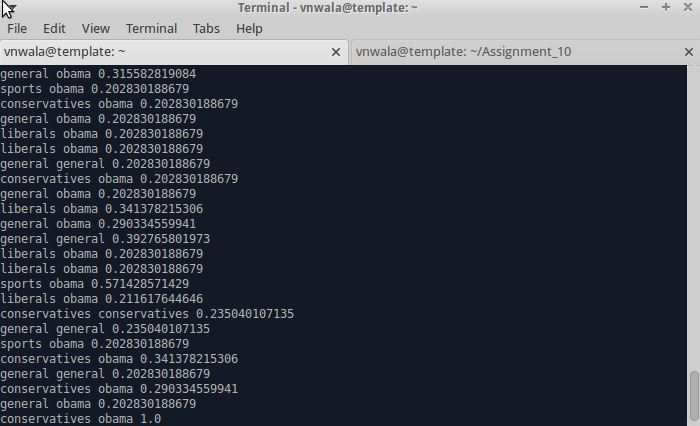
\includegraphics[width=0.75\columnwidth]{testing} % Example image
\end{center}


}
\end{homeworkProblem}


\newpage
%----------------------------------------------------------------------------------------
%   PROBLEM 3
%----------------------------------------------------------------------------------------

\begin{homeworkProblem}
3.  Assess the performance of your classifier in each of your categories
by computing precision, recall, and F1.  Note that the definitions
of precisions and recall are slightly different in the context of
classification.

I predicted 47 out of the 50 classes
For General TP = 4, FP = 0, FN = 43, TN = 28,
For Obama TP = 5, FP = 33, FN = 14, TN = 42,
For Liberals TP = 0, FP = 0, FN = 47, TN = 38,
For Conservatives TP = 2, FP = 0, FN = 45, TN = 38,
For Sports TP = 0, FP = 0, FN = 42, TN = 47.


\begin{center}
    \begin{tabular}{ | p{7cm} | c | c | c |}
    \hline
    Class & Precision & Recall & F1  \\ \hline
    General & 1 & 0.085 & 0.1569 \\
    Obama & 0.13157 & 0.26315 & 0.1754 \\
    Conservatives & 1 & 0.046 & 0.0816 \\
    Liberals & 0 & 0 & 0 \\ 
    Sports & 0 & 0 & 0 \\ \hline
   \end{tabular}
\end{center}  
Also calculating the accuracy of the classification of the model with the formula 
ACC = (TP + TN)/(TP +FP + FN + TN) , it can be multiplied by 100 to give a percentage, I got the following results.

\begin{center}
    \begin{tabular}{ | p{7cm} | c |}
    \hline
    CLASSIFICATION  & PERCENTAGE ACCURACY  \\ \hline
    General & 42.66 \\
    Obama & 50 \\
    Conservatives & 47.05 \\
    Liberals & 44.7 \\ 
    Sports & 52.8 \\ 
    Average Accuracy  & 47.44 \\ \hline
   \end{tabular}
\end{center} 

The average accuracy of my model is less than 50 percent.
\end{homeworkProblem}

\newpage
%----------------------------------------------------------------------------------------
%   PROBLEM 4
%----------------------------------------------------------------------------------------
\begin{homeworkProblem}


Redo questions 2 \& 3, but with manually train 90 entries and 
then classify the remaining 10.


\begin{center}
    \begin{tabular}{ | p{7cm} | c | c | c |c|}
    \hline
    Title & String & Actual & Prediction & cprobValue \\ \hline
read stuff, you should&happy birthday to <a&general&general&0.203045685279\\
impeachment!&well, not the presid&conservatives&obama&0.377358490566\\
read stuff, you should&happy birthday to <a&general&obama&0.304099918545\\
gridlock/polarization&national journal is &conservatives&obama&0.189317106153\\
what are republicans thinking on filibusters?&at this point in the&conservatives&obama&0.203045685279\\
read stuff, you should&happy birthday to <a&general&general&0.203045685279\\
why i expect nothing out of bauer-ginsberg&sparked by my dismis&obama&obama&0.377358490566\\
plain blogger smackdown&<div class="tr\_bq\">o&general&obama&0.322686862035\\  \hline
   \end{tabular}
\end{center} 

\begin{center}
    \begin{tabular}{ | p{7cm} | c | c | c |}
    \hline
    Class & Precision & Recall & F1  \\ \hline
    General & 1 & 0.25 & 0.4 \\
    Obama & 0.1667 & 0.333 & 0.1538 \\ \hline
   \end{tabular}
\end{center} 
The rest of the classes have zero Precision, Recall and F1 values

\end{homeworkProblem}


Concluding this assignment, I received some help from Alexander Nwala. Also some of the string fields in my table are not readable because it is just a part of a whole, all tuples in my table are unique.


%----------------------------------------------------------------------------------------

\end{document}